\section{Technische Realisierung}

\subsection{Eingesetzte Entwurfsmuster}
\subsubsection{Mediator Pattern - Der Text Transfer Agent}
Neben der Verwaltung von klienten- und wohngruppenspezifischen Daten ist die Überführung von Textstücken aus verschiedenen Teilen des
Dokumentationsprogramms die Hauptfunktion der \EBP. Diese Funktion wird im folgenden \textit{Text Transfer} genannt. \newline
Der \textit{Text Transfer} soll aus den Masken Bewohner$\rightarrow$Protokoll, Bewohner$\rightarrow$Projekt und Wohngruppe$\rightarrow$Gruppenbuch
erfolgen. Gespeichert werden die Textfragmente in den verschiedenen Feldern der Betreuungsplanung eines beliebigen Bewohners. Die Unterschiedlichkeit
der Quellen für die zu transferierende Textfragmente und die Variation an Zielfelder war die Schwierigkeit bei der Implementierung dieser
Funktionalität. Da die Anzahl an Objekten, die als Quelle dienen, im Programmverlauf stark variieren kann, muss der Lösungsansatz sehr flexibel
implementiert sein. Abbildung \ref{unstrukturiert} zeigt die Vielzahl an möglichen Kommunikationswegen zwischen den einzelnen Objekten.\\
\begin{figure*}[htp!]
	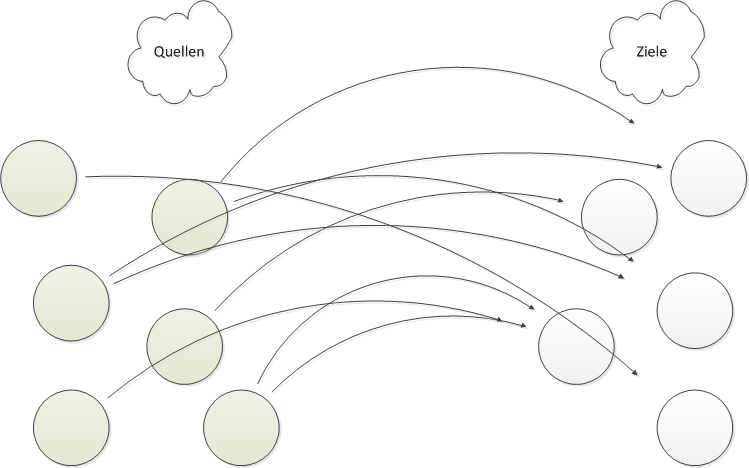
\includegraphics[width=0.8\textwidth]{unmediated}
	\caption{Kommunikationswege zwischen den Objekten}
	\label{unstrukturiert}
\end{figure*}
Um nicht jeden Kommunikationsweg einzeln verwalten zu müssen, wurde der \textit{Text Transfer} in Form des Mediator Patterns entworfen. Den Zweck
eines Mediators definiert GAMMA wie folgt: \\
``Definiert ein Objekt, welches das Zusammenspiel einer Menge von Objekten in sich kapselt. Vermittler fördern lose Kopplung, indem sie Objekte davon
abhalten, aufeinander explizit Bezug zu nehmen. Sie ermöglichen es Ihnen, das Zusammenspiel der Objekte von ihnen unabhängig zu
variieren \cite[S. 385]{Entwurfsmuster}.''\\
Auf einen abstrakten Mediator wird hier verzichtet 

\begin{figure*}[htp!]
	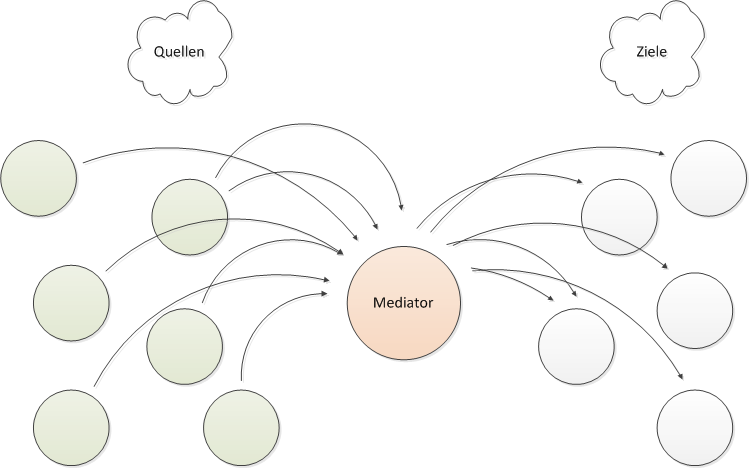
\includegraphics[width=0.8\textwidth]{mediated}
	\caption{Kommunikationswege zwischen den Objekten, koordiniert durch einen Mediator}
	\label{strukturiert}
\end{figure*}
\subsubsection{Observer Pattern - Signal Slot Konzept}
\subsubsection{Model View Controller Pattern - Datenvisualisierung}

\subsection{Architektur}
\subsubsection{Aufteilung der Module}
\subsubsection{Buildsystem}

\subsection{Qt als Grafikbibliothek}

\newpage

\subsection{Persistenzschicht mit ODB (libEBPdb)}

\subsubsection{Object-Relational-Mapping (ORM)}
Um die Daten einer relationellen Datenbank auf Objekte innerhalb einer Programmiersprache abzubilden gibt es prinzipiell zwei Ansätze.
Entweder wird der Code der die Eigenschaften eines Objekts aus der Datenbank liest und schreibt manuell implementiert, oder aber es wird ein Mechanismus eingesetzt, der automatisiert Variablen eines Objekts den Feldern einer Datenbank zuordnet (Object-Relational-Mapping).\\
Das Einsetzen eines solchen Mappers hat den Vorteil, dass der sich oft wiederholende Code zum Laden und Speichern der Daten von und in die Datenbank reduziert werden kann. Dies führt zu wartbarerem Code, der bei Änderungen an der Datenbankstruktur schneller und fehlerfreier anpassbar ist.

\subsubsection{Auswahl des Verwendeten Mappers}
Das verwendete Qt4-Toolkit enthält zwar eine plattformunabhängige Schnittstelle für Datenbanken (QtSql), jedoch hat diese keine ORM Funktion.
Folgende ORM-Systeme wurden in Betracht gezogen\\
\url{http://en.wikipedia.org/wiki/List_of_object-relational_mapping_software}:
\begin{itemize}
	\item LiteSQL - Datenbankschema wird mit XML Dateien beschrieben
	\item ODB - Datenbankschema wird aus den C++ Klassen generiert
	\item QxOrm - Benutzt QtSql; Unter Umständen müssen direkte Aufrufe von QtSql erfolgen. \cite{QxOrm_Tutorial}
\end{itemize}
Alle Systeme bieten eine Qt Integration, die die Schnittstelle zwischen GUI und Persistenzschicht vereinfachen.
Ebenso unterstützen alle Systeme mehrere Datenbankbackends.
Letztendlich fiel die Entscheidung auf ODB, da diese Bibliothek (unter anderem durch Caching) die beste Performance verspricht.
Außerdem lassen sich Klassen mit geringem Aufwandt persistent machen.

\newpage

\subsubsection{Code-Generierung}
Kern des verwendeten Object-Relational-Mappers ODB ist ein spezieller Precompiler, der auf bestimmte Precompiler-Pragmas reagiert.
Durch das Markieren einer Klassendefinition mit einer Pragma-Direktive können persistente Objekte der Klasse erstellt werden:\\
\begin{lstlisting}
#pragma db object
class Mitarbeiter { ... }
\end{lstlisting}
Der ODB-Compiler generiert daraufhin Code, der das gegebene Objekt auf eine Datenbankstruktur abbilden kann. Des weiteren wird auch die Datenbankstruktur in Form von SQL-Dateien generiert, die direkt an die verwendete Datenbank weitergereicht werden können um alle zur Laufzeit benötigten Tabellen zu erstellen. Auf diese Weise wird ebenso sichergestellt, dass Datenbank und Anwendung stets die selbe Struktur verwenden.\\
\begin{figure*}[htp!]
	\begin{center}
		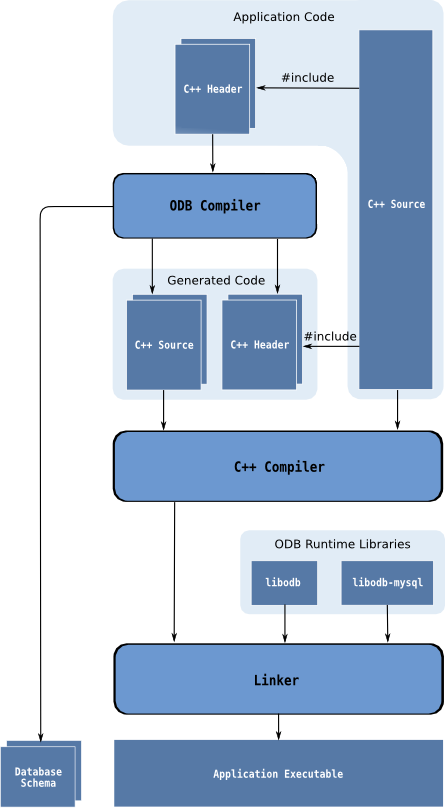
\includegraphics[width=0.4\textwidth]{odb-flow}
	\end{center}
	\caption{ODB Toolchain \cite{ODB_Manual}}
	\label{ODB-Flow}
\end{figure*}

\newpage

\subsubsection{Datenbankunabhängigkeit}
Durch die zusätzliche Abstraktionsschicht ist es einfacher die bestehende Persistenzschicht auf ein neues Datenbanksystem zu portieren.\\
Die umgesetzte Lösung ist weitestgehend frei von datenbankspezifischen Aufrufen, und benutzt ausschließlich die Schnittstelle des eingesetzten Object-Relational-Mappers.
Lediglich das User-Management, um ``Mitarbeiter`` auf Datenbankbenutzer abzubilden verwendet Datenbankspezifische SQL-Kommandos, die über ODB abgewickelt werden.

\subsubsection{Integration in das Buildsystem}
Um das Buildsystem (CMake) automatisch bei veränderungen des Quellcodes alle für ODB benötigten Dateien generieren zu lassen, wird im Buildscript wie folgt vorgegangen:
\begin{enumerate}
\item Suchen aller Dateien die ODB spezifische Pragma-Definitionen beinhalten.
\item Erstellen einer Vorschrift um für jede so gefundene Datei den ODB-Compiler aufzurufen.\\
	Dabei werden auch die Abhängigkeiten der generierten Dateien korrekt in das Buildsystem eingefügt, so dass diese nur neu generiert werden, wenn tatsächlich Änderungen an der jeweiligen Eingangsdatei vorhanden sind.
\end{enumerate}

\newpage

\subsubsection{Datenbankschema}
\begin{figure*}[htp!]
	\begin{center}
		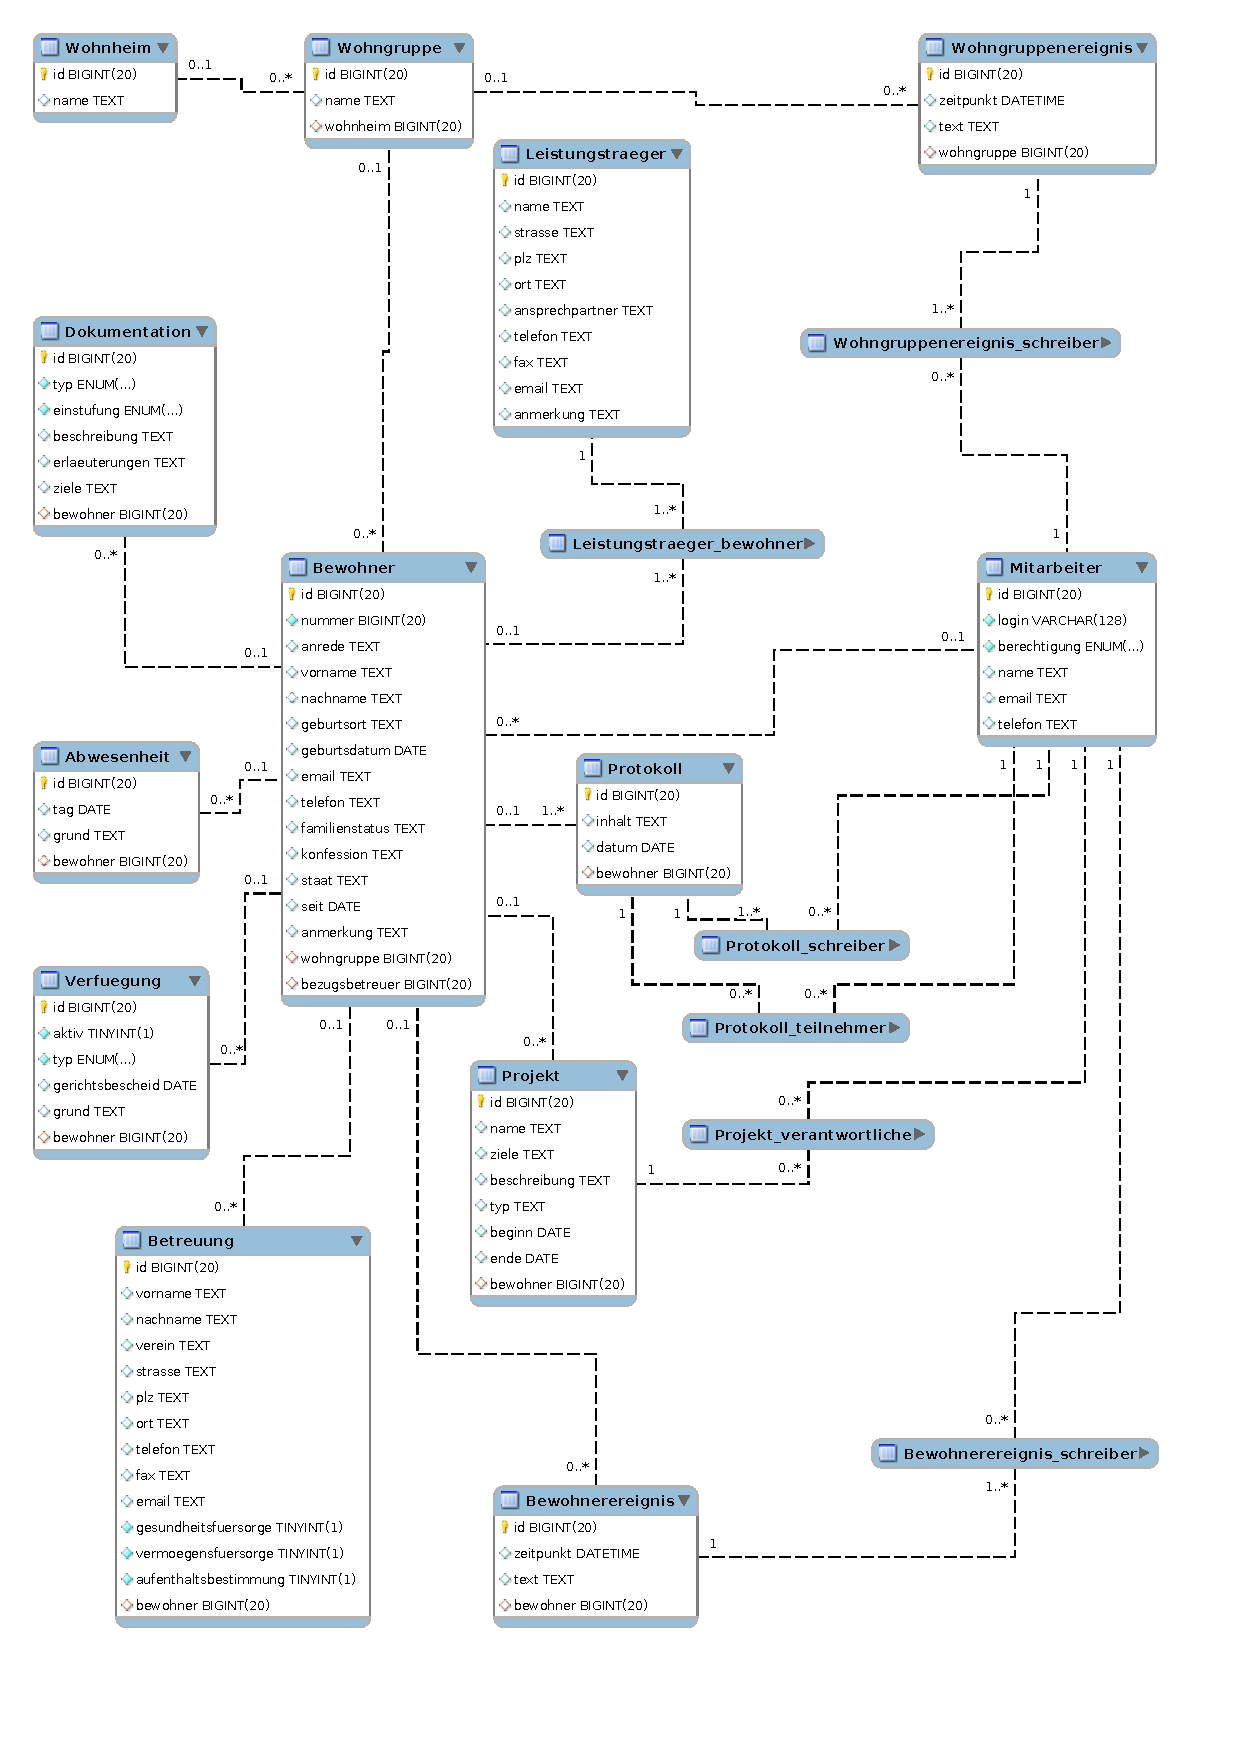
\includegraphics[width=0.93\textwidth]{scheme}
	\end{center}
	\caption{Datenbankschema als ER Diagramm}
	\label{ERDiagram}
\end{figure*}

\subsubsection{Abstraktion der Schnittstelle}
Zweck der Bibliothek ist es die internen Abläufe des ORM Systems zu verbergen, und der Anwendung eine einfache, objektorientierte Schnittstelle zur Verfügung zu stellen.\\
So lässt sich mit\\
\begin{lstlisting}
QSharedPointer<ebp::Mitarbeiter> mitarbeiter =
	QSharedPointer<ebp::Mitarbeiter>
	(
		new ebp::Mitarbeiter( "LoginName", ebp::Mitarbeiter::WohngruppenRecht , "Name" )
	);
mitarbeiter->create( connection, "Passwort" );
\end{lstlisting}
ein neuer Mitarbeiter in der Datenbank erstellen. Gleichzeitig wird auch ein neuer Datenbankbenutzer angelegt, der intern mit den Daten des Mitarbeiters verknüpft wird.
Der Datenbankbenutzer erhält dabei nur die Berechtigungen an den Datenbanktabellen, die er für seinen ''Rechtestatus`` benötigt.
